\documentclass[11pt]{article}
\renewcommand{\baselinestretch}{1.20} 
\usepackage[utf8]{inputenc}
\usepackage[danish]{babel}\addto\captionsenglish  
{\renewcommand{\bibname}{References}}
\setlength\parindent{0pt} % No indent command

% Getting packages
\usepackage[superscript,biblabel]{cite}
\usepackage{url}
\usepackage{csquotes}
\usepackage{hyperref}
\usepackage{subcaption}
\usepackage{pdfpages}
\usepackage[labelfont=bf,labelsep=quad,font={small,it}]{caption}
\usepackage{geometry}
\usepackage{float}
\usepackage{lastpage}
\usepackage{fancyhdr}
\usepackage{titlesec}
\usepackage{booktabs}% http://ctan.org/pkg/booktabs
\usepackage{graphicx}
\graphicspath{ {Projectdoc/Problemanalyse/Illustrationer/} }
\usepackage{wrapfig}
\newcommand{\tabitem}{~~\llap{\textbullet}~~}

\usepackage{url}
\def\UrlBreaks{\do\/\do-\do_}

% Other
\geometry{a4paper, total={170mm,237mm}, left=20mm, top=30mm}
\definecolor{aaublue}{RGB}{33,26,82}
\newcommand{\aautitlepage}[3]{%
  {
    %set up various length
    \ifx\titlepageleftcolumnwidth\undefined
      \newlength{\titlepageleftcolumnwidth}
      \newlength{\titlepagerightcolumnwidth}
    \fi
    \setlength{\titlepageleftcolumnwidth}{0.5\textwidth-\tabcolsep}
    \setlength{\titlepagerightcolumnwidth}{\textwidth-2\tabcolsep-\titlepageleftcolumnwidth}
    %create title page
    \thispagestyle{empty}
    \noindent%
    \begin{tabular}{@{}ll@{}}
      \parbox{\titlepageleftcolumnwidth}{
        \iflanguage{danish}{%
          
\includegraphics[width=\titlepageleftcolumnwidth]{Projectdoc/Assets/Illustrationer/aau_logo_da.pdf}
        }{%
          
\includegraphics[width=\titlepageleftcolumnwidth]{Projectdoc/Assets/Illustrationer/aau_logo_en.pdf}
        }
      } &
      \parbox{\titlepagerightcolumnwidth}{\raggedleft\sf\small
        #2
      }\bigskip\\
       #1 &
      \parbox[t]{\titlepagerightcolumnwidth}{%
      \textbf{Abstract:}\bigskip\par
        \fbox{\parbox{\titlepagerightcolumnwidth-2\fboxsep-2\fboxrule}{%
          #3
        }}
      }\\
    \end{tabular}
    \vfill
    \iflanguage{danish}{%
      \noindent{\footnotesize\emph{Rapportens indhold er frit tilgængeligt, men offentliggørelse (med kildeangivelse) må kun ske efter aftale med forfatterne.}}
    }{%
      \noindent{\footnotesize\emph{The content of this report is freely available, but publication (with reference) may only be pursued due to agreement with the author.}}
    }
    \clearpage
  }
}

%Create english project info
\newcommand{\englishprojectinfo}[8]{%
  \parbox[t]{\titlepageleftcolumnwidth}{
    \textbf{Title:}\\ #1\bigskip\par
    \textbf{Theme:}\\ #2\bigskip\par
    \textbf{Project Period:}\\ #3\bigskip\par
    \textbf{Project Group:}\\ #4\bigskip\par
    \textbf{Participant(s):}\\ #5\bigskip\par
    \textbf{Supervisor(s):}\\ #6\bigskip\par
    \textbf{Copies:} #7\bigskip\par
    \textbf{Page Numbers:} \pageref{LastPage}\bigskip\par
    \textbf{Date of Completion:}\\ #8
  }
}

%Create danish project info
\newcommand{\danishprojectinfo}[8]{%
  \parbox[t]{\titlepageleftcolumnwidth}{
    \textbf{Titel:}\\ #1\bigskip\par
    \textbf{Tema:}\\ #2\bigskip\par
    \textbf{Projektperiode:}\\ #3\bigskip\par
    \textbf{Projektgruppe:}\\ #4\bigskip\par
    \textbf{Deltager(e):}\\ #5\bigskip\par
    \textbf{Vejleder(e):}\\ #6\bigskip\par
    \textbf{Oplagstal:} #7\bigskip\par
    \textbf{Sidetal:} \pageref{LastPage}\bigskip\par
    \textbf{Afleveringsdato:}\\ #8
  }
}

\pagestyle{fancy}
\fancyhf{}
\rhead{Social hidden Messages 2018}
\lhead{Gruppe: B-125}
\chead{P2 - Rapport}
\rfoot{Side \thepage}

\setcounter{secnumdepth}{4}

\titleformat{\paragraph}
{\normalfont\normalsize\bfseries}{\theparagraph}{1em}{}
\titlespacing*{\paragraph}
{0pt}{3.25ex plus 1ex minus .2ex}{1.5ex plus .2ex}

\title{
    P2 - Hidden messages through the media 
    \\ 
    Gruppe: B-125
    \\
    \begin{figure}[!h]
        \centering
        
\includegraphics[width=0.8\textwidth, angle =0]{Projectdoc/Egg-Message.jpg}
        \label{fig:FrontPage}
    \end{figure}
}

\author{
    Udarbejdet af:\\
    \\
    Mikkel Steen Hansen\\
    Martin Boe\\
    Benjamin Jensen\\
    Daniel Jensen\\
    \\\\
    Vejledere:\\ 
    \\
    Rasmus Løvenstein Olsen\\
    Julie Rafn Abildgaard\\
}
\date{\textbf{\today}}

%\addbibresource{references.bib}  

\begin{document}
    % Forside
    \begin{titlepage}
        \clearpage
        \maketitle
        \thispagestyle{empty}
    \end{titlepage}
    
    % Titelblad
    {\selectlanguage{danish}
\aautitlepage{
  \danishprojectinfo{% Rapporten titel:
    Hidden messages through the media
  }{% Temaet:
    Netværksbaseret databehandling
  }{% Projektperiode:
    Forårssemestret 2018
  }{% Projektgruppe:
    B125
  }{% Gruppemedlemmer:
    Mikkel Steen Hansen\\
    Martin Boe\\
    Daniel Benjamin Vestergaard Jensen\\
    Benjamin Bach Jensen
  }{% Vejleder(e):
    Rasmus Løvenstein Olsen\\
    Julie Rafn Abildgaard (Bi-vejleder)
  }{% Printet kopier / Opslagstal:
    1
  }{% Afleveringsdato:
    \today
  }%
}{% Institut adresse:
  \textbf{Institut for Elektroniske Systemer}\\
  Fredrik Bajers Vej 7\\
  DK-9220 Aalborg Ø\\
  \href{http://es.aau.dk}{http://es.aau.dk}
}{% Abstract:
  Her er resuméet
}}

    
    % Indholdsfortegnelse
    \renewcommand{\baselinestretch}{0.8} 
    \tableofcontents
    \renewcommand{\baselinestretch}{1.20} 
    \newpage
    
    %%%%%%%%%%%%%%%%%%%%%%%%%%%%%%%%%%%%%%%%%%%%%%%%
    % Rapport struktur
    %%%%%%%%%%%%%%%%%%%%%%%%%%%%%%%%%%%%%%%%%%%%%%%%
    
    % Læsevejledning
    %\section{Læsevejledning}
Kære læser,

Du vil komme til at læse rapportens nuværende indledning, problemanalyse, problemafgræsning og problemformulering. Du bedes især lægge fokus på transformationen fra vores initierende problemformulering til den endelige problemformulering. Vi ønsker at vide om vorvidt vi har formidlet den proces i problemanalysen/afgrænsning godt. Er der områder vi ikke har belyst eller har sprunget for let over?
\newpage
    
    % Indledning
    \section{Indledning}
Siden mennesket har kunne kommunikere med hinanden, har det også haft behov for at skjule en sandhed eller et budskab. \cite{PastCryptography} Dog har nogle af disse hemmeligheder også senere haft brug for enten at blive gemt, eller delt mellem enkelte individer. Problemet opstår her i, at en nedskreven hemmelighed har lettere ved at blive røbet, og at delingen af denne også kan komme til ikke tiltænkte individer.
Derfor har man altid arbejdet i at kunne kryptere, formatere, eller med andre ord skjule, beskeder til alle tænkelige former for brug, lige fra militante strategier, til deling af videns-studier. \cite{The_Invention_of_the_Internet} \\
Hertil er det dog vigtigt, at være klar over at kryptologi, som betyder "læren om det hemmelige", er et paraplyudtryk. Inden under dette hører blandt andre kryptografi, som nok er den mest kendte sikkerheds foranstaltning, og som er grundlaget for at skjule indeholdet af en besked. Et andet koncept, som hører under kryptologi er steganografi. Dette er anderledes i det, at steganografi handler om, at skjule eksistensen af en besked i stedet for indholdet.\cite{MeningOfCryptography} \quad \cite{MeningOfSteganografi}
I dag arbejdes der stadig hårdt på at udvikle nye metoder til at skjule meddelelser, faktisk med nutidens udbredelse af netværksbaseret løsninger, har behovet for disse metoder af datasikringer aldrig været større.\cite{Internetsikkerhed_forlav} Næsten alle i de industrialiseret lande er i dag online, på det ene eller det andet sociale medie, og selv små lande er igennem internettet eksponeret til resten af verdenen. Da kommunikation over internettet involverer flere elementer end blot de to endpoints, passer dette også godt ind i det overordnede semestertema, som er netværksbaseret databehandling.
    
    % Problemanalyse
    \section{Problemanalyse}
I denne moderne tid, hvor massive mængder af kommunikation foregår over internettet, har det aldrig været nemmere at kommunikere med andre mennesker i verdenen. Netop på grund af denne store mængde og tilgængeligheden af digital kommunikation, er internettet også overvåget i en historisk uset grad. Dette betyder, at kommunikation aldrig har været nemmere, men heller aldrig før har så mange kunne følge med i samtaler der ikke vedrører dem.\cite{Adgang_PersonligeData} På trods af dette er de teknologiske muligheder for at skjule kommunikation store, men ikke realiseret til deres fulde potentiale. Overvågningen bliver dog skubbet til det yderste. Som et led i at undgå en fremtid med totalitære styrer som besidder al information, kræves et modspil som kan genvinde friheden på internettet, og dermed friheden i verdenen. 

Den største kommunikationsplatform i verden på nuværende tidspunkt er, det sociale netværk, Facebook med sine 2.129 milliarder af månedlige aktive brugere gennemsnitligt i løbet af 4. kvartal 2017.\cite{FacebookStat} Facebook har med sin enorme brugerbase, vakt en sådan interesse fra diverse regeringer, bl.a. omhandlede agtindsigt i brugerdata. En rapport fra Facebook selv i 2013, beskrev hvordan de i mindst 80 procent af tilfældene amerikas regering efterspørger brugerdata, få de det udleveret.\cite{PolitikenFacebook} Andre store sociale netværk som Twitter og LinkedIn, har rapporteret lignede forhold.\cite{PolitikenFacebook}

Dette leder frem til den initierende problemformulering:
\begin{quote}
    \textit{Hvordan kan man lave en sikker kommunikationsplatform uden at kommunikationen bliver udsat for overvågning fra uvedkommende?}
\end{quote}

\newpage
%\subsection{Hemmelig kommunikation}
I dette afsnit vil der blive kigget på, hvordan man tidligere har anvendt kryptografi, for at skabe en basal forståelse for hvordan kryptering, eller kryptografi, er blevet til den teknologi der kendes i dag, samt hvilke fordele eller ulemper der kan tages til videre overvejelser.
\subsubsection{Oldtidens hemmelige kommunikation}
\begin{wrapfigure}{r}{0.53\textwidth}
    \vspace{-30pt}
    \begin{center}
        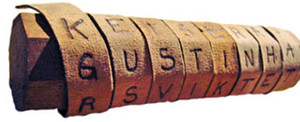
\includegraphics[width=0.75\linewidth]{Projectdoc/Problemanalyse/Illustrationer/scytale.jpg}
    \end{center}
    \caption{En spartansk scytale. Den hemmelige besked skrives på langs med cylinderen mens læderet er omviklet. Beskeden kan så først aflæses når læderet omvikles en lignende cylinder.}
    \vspace{-30pt}
    \label{fig:scytale}
\end{wrapfigure}
% Et af de første daterede kryptografi metoder blev opfundet og anvendt af spartanerne ca. 500 år før kristifødsel. \\
Et af de første daterede metoder indenfor hemmelig kommunikation blev opfundet og anvendt af spartanerne ca. 500 år før kristifødsel. \\
Denne metode "Den Spartanske scytale [Se Figur: \ref{fig:scytale}]" banede vejen for, hvad vi i dag kender, da denne opfindelse var en af de første, der ikke blot anvendte lokale metoder, så som sprog, men et faktisk værktøj og algoritme til at transponere kendte tekster til kode.\cite{PastCryptography}
%Den spartanske scytale var nemlig en cylinder, hvorom man viklede noget at skrive på, herefter skrev man sin besked på de enkelte sider, således når man fjernede cylinderen kunne man ikke forstå sammenhængen, før man havde en cylinder i samme størrelse.
%, dog findes også andre eksempler på mere avancerede anvendelse af værktøjer, så som kryptograferings maskinen "Enigma" fra Den Anden Verdens krig.\cite{PastCryptography}

\subsubsection{Hashings algoritmens forgænger}
Ca. 500 år efter den Spartanske scytale opfandt man i Rom, hvad der i dag er den mest kendte og brugte transponerings kryptografi "A-K Koden".
%\\A-K Koden går i alt sin simpelhed ud på, at man flytter alfabetet en vis grad, f.eks. i A-K ville "ABCD" skrives "KLMN", eller i A-S ville "ABCD" skrives "STUV".
\cite{TheSecretLanguage}\\
Denne krypterings metode har siden sin oprindelse været brugt i et større antal af nyopfundne metoder, 
%ikke kun pga. dens simpelthed og meget store aspekt af kombinationer, men også
mest grundet at den er grundlaget for alt fra simple algoritmer til de sværeste algoritmer. 
Faktisk kan man i flere af de nu-tids største datakrypterings algoritmer, også se en bassering på noget ligende en længere form af "A-K Koden", som man stadig udregner flere af. 
Dog er A-K Kodens største svaghed også dens udbredelse. Da denne kode i dag er kendt verden over, og efter anvendelse danner et ikonisk rod af usammenhængende bogstaver, der nemt ville genkendes som transformeret data, er denne metode også en af de først anvendte, i forskellige former, hvis en tredjepart skulle de-kryptere.

\subsubsection{Den nyere tids kryptografi}
Faktisk er A-K Koden så alment anvendt, at der kun findes et mindretal af nye og anderledes kryptografi former. Et eksempel på et sådant kunne dog være "Morse Koden" opfundet i 1836. Morse koden anvendte nemlig som andre former end kun tekst, men i stedet også lyd. 
%Lyden blev sendt gennem den datid revolutionerende telegraf og dens netledninger, også i vores tid kendt som telefonnettet.
\cite{Telegraphing} Denne nye idé at skjule ikke blot en handling, men også selve dens eksistens som støj, kan siges at have været en større mulighed, hvis ikke dens udførelse havde været så udbredt, at den i dag danner kendte ikoniske træk. F.eks. Vil de fleste i dag kunne genkende et "S.O.S".

\subsubsection{De legendariske steganografier}
Som nævnt i indledningen, så består emnet kryptologi af flere underkategorier. Den kategori der vil blive fokuseret mest på her, er steganografi. Dette omhandler metoder til at skjule selve eksistensen af en given besked, i stedet for at gøre indeholdet ulæseligt, som er hvad kryptografi.\cite{MeningOfSteganografi} Et eksempel på beskeder der er sikret med steganografi vil være de hemmelige signaler som der bruges af spioner i film. Et tilsyneladende tilfældigt symbol på et umiddelbart ligegyldigt sted, er blot en af de mange forskellige ting som kunne sende en besked sikkert frem. Alt dette vil foregå imens ingen andre vil opdage, at der overhoved var en form for kommunikation. Udenfor fiktion findes der også nogle eksempler på grupper som har udviklet systemer baseret på steganografi til at kommunikere internt.
%kommunikere internt. Fra kryptografiernes modsætningt  findes steganografi. Hvor kryptografi altid har været mere eller mindre alment kendt, er steganografier for det meste kun anvendt i mindre data baserede emner, og er derfor ikke udbredt eller kendt i lige så stort et omfang.
% Dog findes steganografi stadig i flere forskellige udformninger, og har blandt andet været anvendt til både handel, men også af f.eks. hjemløse.
\begin{figure}[H]
    \begin{subfigure}{0.5\textwidth}
    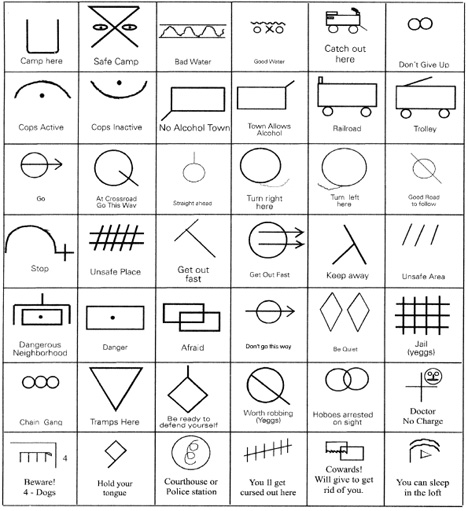
\includegraphics[width=0.9\linewidth, height=5cm]{Projectdoc/Problemanalyse/Illustrationer/hobo-glyphs-code.jpg} 
    \caption{The Hobo Code}
    \label{fig:hobocode}
    \end{subfigure}
    \begin{subfigure}{0.5\textwidth}
    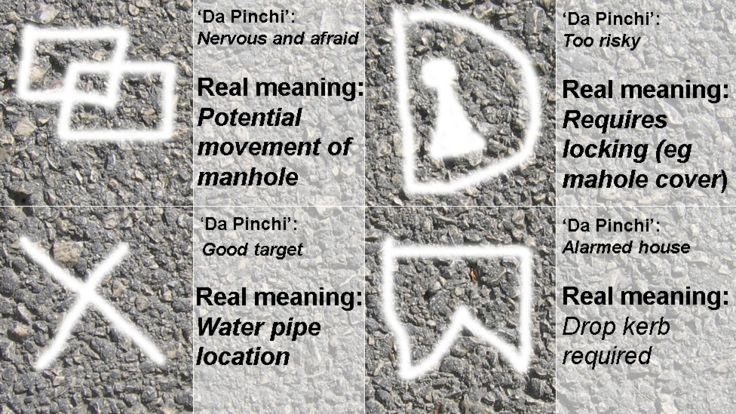
\includegraphics[width=0.9\linewidth, height=5cm]{Projectdoc/Problemanalyse/Illustrationer/BurglarsCode.jpg}
    \caption{Da Pinchi Code / The Burglars Code}
    \label{fig:burglarscode}
    \end{subfigure}
    \caption{To af de legendariske kryptografi metoder}
    \label{fig:legendscode}
\end{figure}
\noindent
Et kendt eksempel på en sådan steganografi metode kunne være "The Hobo Code [Se Figur: \ref{fig:hobocode}]", en bestemt del af kryptologien kendt, og anvendt, af hjemløse til at hjælpe hinanden med deres overlevelse\cite{TheHoboCode}. Disse beskeder er aldrig rigtigt blevet dateret, og ingen i dag kender derfor deres præcise oprindelse, men det vides dog stadig at denne kryptologiske metode har været anvendt i flere århundrede.\\ 
Foruden videnen om metodens eksistens gennem årene, vides også at der findes flere andre ligende afarter af denne kendte kode, såsom den nytidiske "Da Pinchi Code [Se Figur: \ref{fig:burglarscode}]". Denne kode bliver alment anvendt af konstruktions arbejdere, men siges også, efter historier, at have været anvendt af indbrudstyve eller andre kriminelle.\cite{DaPinchiCode}

\subsubsection{Anvendelsen}
Dette faktum at der findes flere steganografiske metoder, der ikke er særligt kendte, som man stadig kan anvende uden at f.eks. politiet aner uråd, giver et indtryk af at man ville kunne anvende ligende metoder i en nyere teknologi og derved muligvis opnå samme effekt. \\
Man prøver i dag ved alle tænkelige metoder at kryptere forbindelser på nettet, hashe data og oplysninger, eller lige frem at danne sikre VPN tunler mellem sender og modtager. Men alle disse har det tilfældes med A-K koden og Morsing, at de er kendte og synlige, og derfor på et eller andet tidspunkt vil deres sikkerhed blive brudt. Men de legendariske steganografiske metoder har alle den vigtige egenskab at de færreste ligger mærke til dem, selvom de befinder sig lige foran dem, midt på den offentlige gade. Disse egenskaber kunne, muligvis ved nærmere studie, blive anvendt til videregivelse af beskeder på F.eks. De åbne sociale medier, så som Facebook, der allerede er kendt for at tilbageholde alle informationer til videregivelse eller studie. Ved andre tilfælde, kunne denne metode måske endda også anvendes til udveksling af information på tværs af modstående lande, så som Rusland og USA.


% -------------------------
% Fra moderne kommunikation
% -------------------------

%\subsection{Moderne kommunikation}
%I det foregående afsnit blev udviklingen af hemmelig kommunikation gennemgået og en bestemt metode, steganografi, blev fremhævet som et muligt værktøj. I dette afsnit vil det blive undersøgt hvorfor og i hvilken udstrækning, at en ny type af hemmelig kommunikation skulle være nødvendig.

\subsection{Sikker kommunikation}
Der vil i dette afsnit blive kigget på hvad det vil sige at kommunikere sikkert, både i levering, men også i håndteringen af kommunikationen. Tilsidst vil der blive konkluderet et grundlag for foretagelse af sikker kommunikation.

\subsubsection{Kryptologi}
De fleste forbinder moderne IT-sikkerhed med avanceret krypteringsalgoritmer. Selvom dette er en vigtig del af IT-sikkerhed, er det dog ikke den eneste måde at sikre kommunikation på. Under emnet kryptologi, som omhandler alle former for hemmelig kommunikation, er kryptografi kun en del af emnet. Et andet vigtigt koncept som også dækker er steganografi, der videre vil blive diskuteret i næste afsnit. Den førnævnte algoritmebaseret sikring af data falder ind under kryptografi. Eksempler på disse spænder fra den simpleste alfabet skiftende algoritme, f.eks. ét bogstav skift til højre, og videre til moderne hashing algoritmer. Fælles for anvendelsen af alle disse er dog, at det tydeligt viser en intention om at hemmeligholde indholdet. Hermed kan selve krypteringen gøre beskeden mistænkelig, da information af lav værdi ikke ville være besværet værd.

\subsubsection{Steganografi}
Som nævnt i indledningen, består emnet kryptologi af flere underkategorier. Den kategori der vil blive fokuseret på her, er steganografi. Steganografi omhandler metoder til at skjule selve eksistensen af en given besked, i stedet for at gøre indeholdet ulæseligt, som er hvad kryptografi gør.\cite{MeningOfSteganografi} Et eksempel på beskeder der er sikret med steganografi, kunne være de hemmelige tegn og signaler, også ofte brugt af spioner i film. Et tilsyneladende tilfældigt symbol på et umiddelbart ligegyldigt sted, men blot en af de mange forskellige ting som kunne sende en besked sikkert frem. Alt dette vil foregå imens ingen andre vil opdage, at der overhovedet var en form for kommunikation. Udenfor fiktionens verden findes der dog også nogle eksempler på grupper, som har udviklet systemer baseret på steganografi til at kommunikere internt.
\begin{figure}[H]
    \begin{subfigure}{0.5\textwidth}
    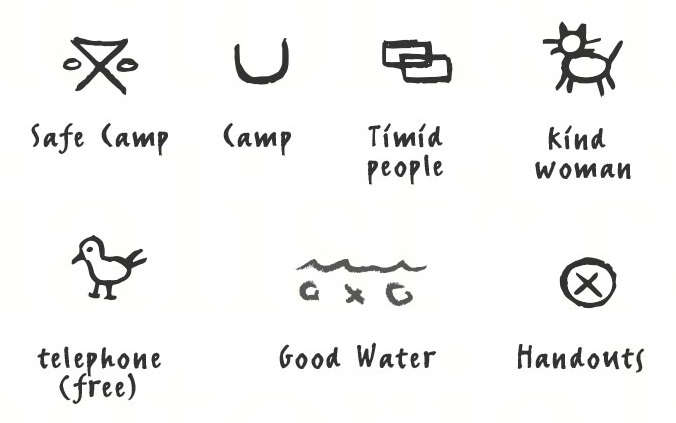
\includegraphics[width=0.9\linewidth, height=5cm]{Projectdoc/Problemanalyse/Illustrationer/hobo.jpg} 
    \caption{The Hobo Code}
    \label{fig:hobocode}
    \end{subfigure}
    \begin{subfigure}{0.5\textwidth}
    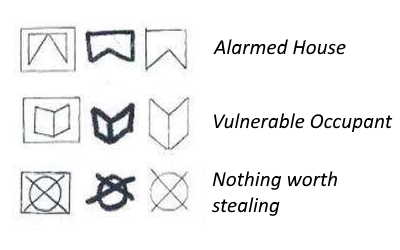
\includegraphics[width=0.9\linewidth, height=5cm]{Projectdoc/Problemanalyse/Illustrationer/da-code.png}
    \caption{Da Pinchi Code / The Burglars Code}
    \label{fig:burglarscode}
    \end{subfigure}
    \caption{To af de legendariske steganografi metoder}
    \label{fig:legendscode}
\end{figure}
Et kendt eksempel på sådan et steganografisk system kunne være "The Hobo Code [Se figur: \ref{fig:hobocode}]", et system kendt, og anvendt, af hjemløse til at hjælpe hinanden med deres overlevelse\cite{TheHoboCode}. Disse beskeder er aldrig rigtigt blevet dateret, og ingen i dag kender derfor deres præcise oprindelse, men det vides dog stadig at dette steganografiske system har været anvendt i flere århundrede.\\ 
Foruden videnen om metodens eksistens gennem årene, vides også at der findes flere andre ligende afarter af denne kendte kode, såsom den nytidiske "Da Pinchi Code [Se figur: \ref{fig:burglarscode}]". Denne kode bliver alment anvendt af konstruktions arbejdere, men siges også, efter historier, at have været anvendt af indbrudstyve eller andre kriminelle.\cite{DaPinchiCode} At lave sikre systemer handler dog ikke kun om den underlæggende teori. Brugerne af systemet kan også lave fejl, eller bruge systemet på ikke tiltænkte måder, som potentielt kunne skade systemet, eller brugerne, som en helhed. Derfor vil der i det næste afsnit diskuteres en sådan brugerbaseret problematik. 

\subsubsection{Brugeren som sikkerhedsbrist}
\label{Brugeren_som_sikkerhedsbrist}
I dag forsøger mange at bibeholde, hvad der for dem synes at være, sikker eller hemmelig kommunikation via diverse tjenester. For nogle er disse tjenester dog mere sikre end hos andre. Som et eksempel vil de fleste private computerbrugere, nok mene at deres generelle email er forholdsvis sikker, men deres arbejdsplads deler muligvis ikke samme overbevisning. Dette var f.eks. tilfældet hos Hillary Clintons email-skandale tilbage i 2015-2016.\cite{Hillary_Email_History} Hillary Clinton havde oprettet sin egen mailserver til håndtering af alle hendes mails, dog mener flere, blandet andet FBI, at denne handling har været en "ekstremt uforsigtigt" håndtering af hendes fortrolighed. Trods Hillarys skandale menes dog ikke at et større sikkerhedsbrud har fundet sted, men Hillary har stadig som bruger mindsket den tilgængelige sikkerhed, i følge FBI, da de mener at hun fejlagtigt har misbrugt det vante system.\cite{Hillary_Email_skandale} Det efterfølgende afsnit vil danne overblik over de vigtigste elementer af sikker kommunikation.

\subsubsection{Grundlaget for sikker kommunikation}
I dag forsøger folk ved alle tænkelige metoder at kryptere forbindelser på nettet, men da kryptering er kendt og synligt, vil det derfor på et eller andet tidspunkt blive, eller være forsøgt, brudt. Steganografiske metoder har til gengæld alle den vigtige egenskab, at ikke alle vil ligge mærke til dem, selvom de befinder sig lige foran dem. Steganografiens egenskaber kan sammen med de sociale mediers endeløse strøm af indhold, fungere som et ekstra lag af sikkerhed. Udover kommunikationens skjulte eksistens, vil den kommunikation være at finde blandt milliarder af uskyldige indlæg.\\
En effektiv implementation af dette, kunne endda sikre kommunikation imellem stridende lande, hvor sikker og åben kommunikation ikke er en selvfølge.
Dog skal man også, for en endelig metode, have i tanke, at jo mere frihed man giver en bruger, jo større er risikoen for, at brugeren anvender systemet på en ikke tiltænkt, eller ligefrem uforsvarlig måde.
\\\\
I det næste afsnit vil nogle udvalgte kommunikationsplatforme blive analyseret baseret på netop disse kriterier.
\newpage
\subsection{Overvågning af kommunikation på nettet}
Der vil i dette afsnit blive kigget på hvordan og hvorfor der foregår overvågning og censur på internettet, samt hvordan det kan omgås.

\subsubsection{Politisk censur}
I 2015 fandt Freedom House, som er en uafhængig frihedskæmpende organisation, frem til, at 15 regeringer ud af de 65 undersøgte, havde begrænset befolkningens adgang til diverse sociale medier.\cite{FreedomHouseRapport2016} Tendensen havde i 2016 vokset sig til 24 regeringer.\cite{FreedomHouseRapport2016} Brasilien og Tyrkiet endte 2016's undersøgelse med, at blive to af de mest bemærkelsesværdige lande, da de begge gik et betydeligt skidt tilbage på deres respektive frihedsskalaer, netop på grund af deres magtanvendelse overfor diverse sociale medier. Brasilien gik fra kategorien "Free" til "Partly Free", da brasilianske domstole indførte en midlertidig blokering af opkald- og tekstkommunikations tjenesten WhatsApp. WhatsApp nægtede nemlig at udlevere brugerdata til bevismateriale. Tyrkiet gik fra kategorien "Partly Free" til "Not Free" efter masseblokeringer af diverse sociale medier, og efterfølgende forfølgelse af borgere, der kritiserede Tyrkiets regering.\cite{FreedomHouseRapport2016}
\\\\
Det kan virke som om at de sociale medier kun er til befolkningens fordel, med eksempler på organisering af store demostrationer og muligheden for at dele beretninger om uretfærdighed fra hele kloden, men regeringerne lytter med. Regeringer er blevet bedre til at manipulere sprede deres politiske agenda på de sociale medier end aktivisterne.\cite{SocialHelpDictators} Det ses blandt andet i Freedom Houses rapport fra 2017, som fandt mindst 18 regeringer der med hjælpe af sociale medier har spredt misinformation og dermed har manipuleret valgenes valg, heriblandt USA.\cite{FreedomHouseRapport2017}


%Det ses stadig i dag hvordan utilfredse befolkninger rundt om i verden kæmper mod uretfærdighed, f.eks under Det Arabiske Forår hvor at en række arabiske lande gjorde op med deres diktatoriske ledelse.\cite{ArabiskeForaar} Under disse oprør, især i nyere tid, har de sociale medier været uvurderlige i at få befolkningsgrupper engageret og oplyst til at ville kæmpe for deres respektive sag. Da disse sociale medier er gode til at få samlet folk, og organisere protester og lignede, vil visse regeringer bruge deres magt på undertrykkelse.
%Det er dog ikke kun aktivisme, nogle af disse autoritære regimer undertrykker også homoseksuelle fællesskab, satire, religiøse- og modstående politiske overbevisninger.
%Disse udsatte grupper har i høj grad brug for at de kommunikationskanaler de benytter beskytter deres kommunikation og oplysninger, sådan de ikke falder i de forkerte hænder.

\subsubsection{National sikkerhed eller privatliv}
En forøgelse i individers private sikkerhed vil også komme kriminelle og terrorister til gavn, da det vil gøre det nemmere for dem at skjule deres intentioner og handlinger.

Nogle stater har endda diskuteret delvis blokering af VPN tjenester for at gøre det sværere for kriminelle at gemme sig. Dette ville dog også påvirke individer der blot vil diskutere landets politiske klima, eller andre emner som de enkelte stater har sat sig imod.
% Metoder til at undgå overvågning, som leder til andre typer overvågning og/eller blokeringer

Et eksempel på konflikten mellem national sikkerhed og privatlivetsfred er bagdøre til krypterede systemer. På den ene side ville denne bagdør blive brugt af regeringer til at fremme efterforskningen af kriminelle. På den anden side kan sådanne bagdøre også anvendes af kriminelle og regeringer som vil undertrykke deres befolkninger. FBI og Apple har været i netop sådanne situationer hvor Apple ikke har ville lave en generel bagdør for, at beskytte deres brugere.\cite{FBI/Apple_encryption}

% Et godt eksempel på dette er de sager hvor FBI har bedt Apple om, at bryde sikkerheden på et af deres egne produkter\cite{FBI/Apple_encryption}. Naivt ville man måske sammenligne dette med at bede en låsesmed om, at åbne en låst dør. Dette er naturligvis inden for hvad politiet forventer at kunne bede om. Problemet er, at analogien i dette tilfælde ikke holder. Det gør den ikke, da man for at bryde cybersikkerhed bliver nød til at skrive noget software, til at kompromittere en bestemt type enhed. Dette stykke software ville så kunne bruges på alle lignende enheder, eller nemt modificeres til dette, og dette er netop problemet. Hvis blot man kunne være sikker på, at denne software aldrig nogen sinde ville blive misbrugt, så ville det principielt være en funktionel løsning. Men det kan man ikke. I kontrast til en fysisk masterkey, hvor fysiske kopier tager tid, penge og ekspertise at producere, så kan en software baseret masterkey kopieres i det uendelige. På den måde går en umiddelbart fornuftig forespørgsel hurtigt over til at have potentielt store og vidt rækkende konsekvenser.\\\\

% En anden sikkerhedsforanstaltning, som diverse regeringer, herunder Kina, Rusland og Egypten\cite{FreedomHouseRapport2017}, ønsker at regulere, er VPN'er eller Virtual Private Networks. En VPN beskytter brugerens privatliv og sikkerhed på nettet, ved at fungere som et ekstra led mellem brugerens enhed og internettet [Se Figur: \ref{fig:vpn}]. Denne forbindelse er krypteret, som betyder at brugerens data og handlinger er sikret.\cite{VPNInfo} Derudover kan en VPN virtuelt skifte den geografiske position af en given enhed, og dermed undgå eventuelle regeringers censur, af for eksempelvis internationale nyhedsbureauer, eller sociale medier. Selvom VPN kan blive brugt til kriminel aktivitet, så bruger de fleste den til godsindet formål, såsom: at værne om privatlivet, forblive informeret via censureret medier, eller blot som et led i deres internationale arbejde. De regeringer der ønsker at regulere VPN'er, vil dog ikke blokerer VPN'erne helt, da de netop bruges af regeringens ansatte, som et essentielt redskab. Regeringerne ønsker en proces, hvor at den enkelte VPN udbyder skal autoriseres til at operere i et given land, ved et sæt defineret brugstilfælde, resten af udbyderne vil blive blokeret af regeringen.\cite{FreedomHouseRapport2017}


% Moderne efterforskning inkluderer i højere grad de forskellige kommunikationskanaler, når kriminalitet og terror aktivitet skal bekæmpes. Smartphone, computere og online services er i vor tid tætpakket med avanceret kryptering, både for at beskytte virksomhedens brugere, men også virksomheden selv. Denne kryptering så myndighederne, i blandt andet Kina, Ungarn, Rusland, Thailand, Storbritannien og Vietnam, gerne gradbøjet, som led i individuelle lov ændringer indefor området. Disse love kan blandt andet kræve at virksomheder udleverer backdoor eller bagdørs krypteringsnøgler til myndighedernes efterretningstjenester. Dette kan udgøre en kolossal risiko for alle brugerene af det pågældende medie, især for de brugere der har brug for en sikker kanal til journalistik, aktivisme osv.\cite{FreedomHouseRapport2017} Det åbner op for at visse regeringer har muligheden for at misbruge brugerne på de sociale mediers data udenfor et efterforsknings miljø, hvilket også er virksomhedernes største frygt i forbindelse med disse bagdøre.\\
\newpage
\subsection{Sikring af kommunikationsplatforme}
For at undersøge hvordan moderne kommunikationsplatforme sikrer deres brugere vil to af de største, Facebooks Messenger og WhatsApp, blive diskuteret. I Messenger appen findes en indstilling til at lave en End to End krypteret chat med én anden person. Hvis man ikke kender til funktionens eksistens, så opdager man den måske ikke. WhatsApp har derimod End to End kryptering aktiveret som standard, også for gruppe chats. Forskellen ligger her i, at den informerede bruger kan kommunikere sikkert over begge platforme, men dette kræver dog, at den enkelte bruger selv aktiverer sikkerheden. Dette medfører i praksis, at en del af bruger basen er mindre sikret kun grundet manglen på kendskab til denne sikkerhedsfunktion. Hvorfor er denne kryptering ikke standard på Messenger, når Facebook også ejer WhatsApp\cite{Facebook_WhatsApp_Merger}, hvor det er standard? Dette kunne være for at undgå potentielle problemer med blokering i visse lande\cite{Facebook_security_features}, så som den førnævnte sag med blokeringen af WhatsApp i Brasilien. Samtidigt kunne de ukrypterede samtaler over Messenger være materiale for deres individuelt tilpassede reklamer.
\\
Herefter vil det være naturligt, at betragte WhatsApp som det rigtige valg til privat kommunikation. Problemet med den konklusion er dog tofoldig. Først kan nævnes at man i nogle lande kunne blive mistænkt for at gemme på noget, kun fordi man bruger en platform med bedre sikkerhed end Messenger. Dette er naturligvis aldrig en god ting. For det andet, bør man også overveje hvordan resten af systemet fungerer. Selvom WhatsApp bruger End to End kryptering så har systemet et antal problemer i følge "Electronic Frontier Foundation"\cite{WhatsApp_Security_Concerns}. Ét af disse problemer er et sikkerhedshul som ligger i muligheden for, at lave backups i Google Drev. Denne feature gør det nemt at skifte til et nyt device. Problemet ligger i det faktum at disse backups ikke er krypteret. En konsekvens af dette er, at alle mange brugers chats kan kompromitteres af én brugers ukrypterede cloud backup. Hermed kommer den enkelte brugers valg af sikkerhedsindstillinger til at påvirke andre brugere, som ikke kan gøre noget for at beskytte sig imod dette problem.
\\
Det kan derfor konkluderes at med to af de mest brugte kommunikationsplatforme, så kan awareness på den enkelte brugers part gøre en forskel, men også at andre brugers mangel på samme også kan have en negativ indflydelse på det velvidende indvid. Individets sikkerhed på en kommunikationsplatform burde ikke være afhængigt af andre brugeres valg af indstillinger.
\newpage
    
    % Problemafgrænsning
    \section{Problemopsamling}
Gennem problemanalysen er det blevet gennemgået og diskuteret, hvordan behovet for at skjule informationer fra uvedkommende, altid har været efterspurgt, og stadig er nødvendig den dag i dag. Det er et relevant emne i dag, at bevare sine personlige informationer samtidig med, at kunne anvende internettet i sikkerhed for overvågning og censur. Dette er blandt andet et problem for brugere af internettet i lande med lavere internetfrihed, så som Tyrkiet og Kina.\cite{FreedomHouseRapport2017}
\\\\
Data sikkerhed er i dag blevet en industriel standard for mange virksomheder, der forstår vigtigheden ved at få sine kunder og brugere til at føle sig sikre. Dette resulterer dog i et øget fokus fra blandt andet kriminelle og myndigheder på disse sikkerheds metoder, og hvordan de kan penetreres. På trods af dette, er data sikkerheden langt fra perfekt, hos de undersøgte kommunikationsplatforme [Se afsnit: \ref{kommunikationsplatforme}].
\\\\
Det er gennem problemanalysen blevet antydet, at den tekniske sikring af kommunikation, ikke blot kan opnås ved at kryptere en besked, men også ved at skjule beskedens eksistens. Selvom en krypteret besked er ulæselig for den uvedkommende, kan der stadig se at her er tale om en form for hemmelig kommunikation, som i sig selv kunne give anledning til blokering fra bl.a. regeringer og lignende. Nogle af de grupper der kan være nødsaget til at kommunikere i al hemmelighed, er blandt andet aktivister, journalister og hackere, både de gode og ondesindet. Disse grupper er særligt udsatte alt efter, hvad de laver, og hvor i verden de befinder sig.\cite{FreedomHouseRapport2017}
\\
Disse grupper kunne derfor drage gavn af en internetbaseret kommunikationsplatform, som kan undgå overvågning, og som ikke vil blive opfattet som værende et forsøg på hemmelig kommunikation. 
Da overvågningen på internettet kan antages at være altdækkende, bliver en oplagt mulighed for at undgå overvågning, at anvende steganografi. Ydermere vil det, grundet de forskellige baggrunde af brugerne, også være væsentligt, at brugerne ikke kan kompromittere dem selv og andre, f.eks. gennem uinformerede beslutninger. [Se afsnit: \ref{Brugeren_som_sikkerhedsbrist}]
    
    % Problemformulering
    \section{Problemformulering}
I denne tid hvor overvågning er blevet så vidtrækkende, er det svært at bevare sine private kommunikationer, uden aflytning eller anden indgriben fra staten eller kriminelle. Derfor vil gruppen undersøge muligheden for at skabe et sikkert medie, hvor brugerne kan sende individuelle eller gruppe sammenhængende beskeder. Dette sikre medie skal lagre og sende de hemmelige beskeder sådan at uvedkommende hverken kan læse beskeden eller ane uråd om den hemmelige beskeds eksistens. 
\\Det udmunder i følgende problemformulering:
\begin{quote}
\textit{Hvordan kan man lave en meddelelsesplatform med fokus på sikkerhed, hvor man kan dele beskeder, som bliver skjult således at det er sværere at opdage deres eksistens?}
\end{quote}

    
    % Metode
    \newpage
\section{Kravspecifikationer}


\section{Metode}
    
    %Konklusion
    \section{Konklusion}
\begin{figure}[H]
    \centering
    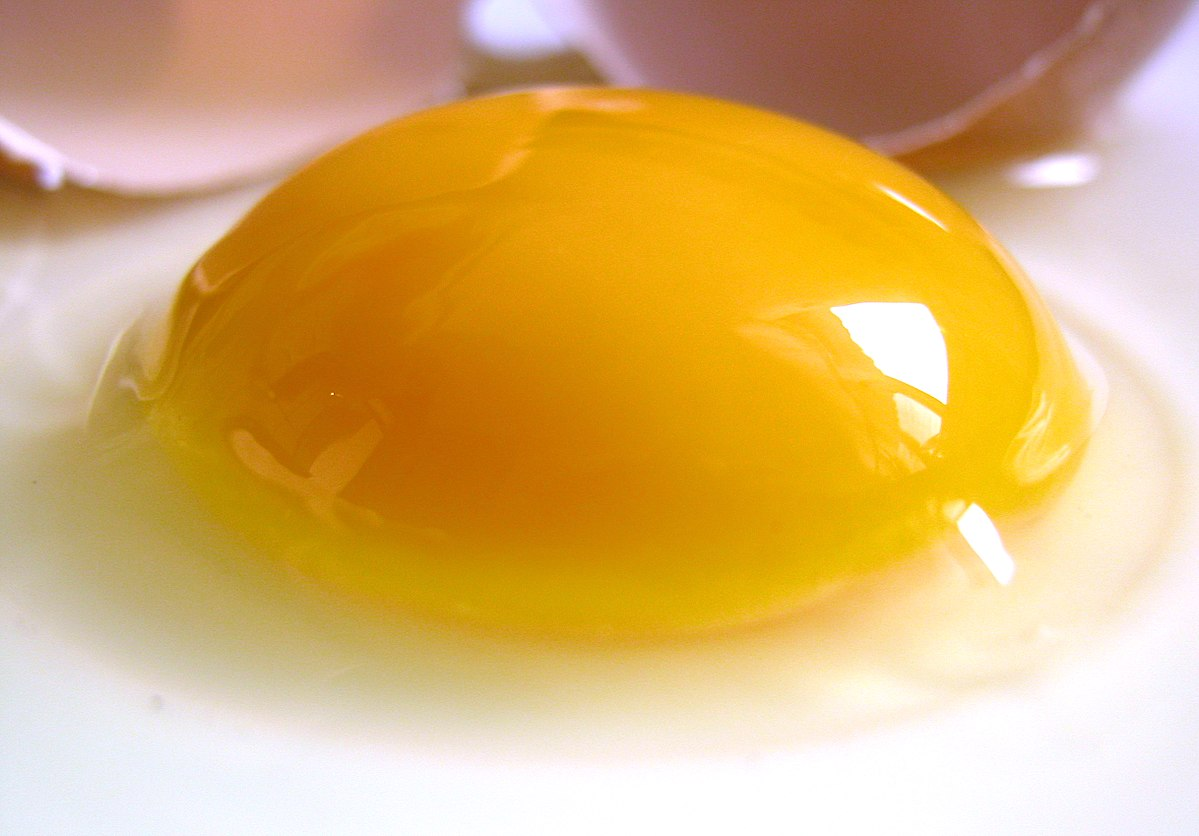
\includegraphics[width=0.70\linewidth]{Projectdoc/Assets/Illustrationer/Egg}
    \caption{System}
    \label{fig:sysdiagram}
\end{figure}
    
    % Litteratur
    \newpage
    \bibliographystyle{unsrt}
    \bibliography{references}
\end{document}